\chapter{System description}
\label{system}

%%%%%%%%%%%%%%%%%%%%%%%%%%%
\section{System overview} %
%%%%%%%%%%%%%%%%%%%%%%%%%%%

The sofware components of the PrologPF system are:
\begin{itemize}
\item{The PrologPF compiler}
\item{The Skynet control processor}
\item{The Skyhub group controller}
\item{The \texttt{ppc} path processor control daemon}
\item{The compiled user program}
\end{itemize}

A diagram of the systems architecture is given in Figure \ref{system_diag}.

\begin{figure}[htbp]
\vspace{5mm} \hbox to \hsize{\hfill \psfig{file={system/ps/system_diag.ps}} \hfill}
\caption{System communications architecture}
\vspace{5mm}
\label{system_diag}
\end{figure}

After compilation of the user program with the PrologPF compiler, the
executable binary is made available to every path processor.  A set of
commands are provided on the control processor to establish communication
between the control processor and the selected number of path processors,
via the intermediate Skyhub processors.  The control processor can then
initiate and control the execution of the user program on every selected
path processor, accumulate statistics, and display the collected results.

%%%%%%%%%%%%%%%%%%%%%%%%%%%%%%%%%%%%%%%%%%%%%%%
\section{The Prolog compiler: \texttt{wamcc}} %
%%%%%%%%%%%%%%%%%%%%%%%%%%%%%%%%%%%%%%%%%%%%%%%

PrologPF is built upon the excellent Prolog to C compiler \texttt{wamcc}
developed by Daniel Diaz at INREA \cite{CD95}.  The \texttt{wamcc} is written
in Prolog, as a series of modules named \texttt{wamcc0.pl} through to
\texttt{wamcc8.pl}.

Starting with a user program \texttt{foo.pl}, the compilation with \texttt{wamcc}
proceeds as follows:
\begin{verbatim}
wamcc -c foo.pl
gcc -c foo.c
gcc -s -o foo -lwamcc
\end{verbatim}
The first compilation step creates two C source files, \texttt{foo.c} and
\texttt{foo.usr}.  The main C file \texttt{foo.c} has definitions to
include the file \texttt{foo.usr} and a number of header files with utility
functions and macros.  The file \texttt{foo.c} is valid C, but closely
resembles WAM code \cite{War83}, with each instruction defined as a C macro.
Each Prolog procedure translates into a preamble and postamble wrapper of C code
enveloping the C macros defining the WAM instructions.

After \texttt{wamcc} has produced the C code, this program can be compiled and
linked with the standard system C compiler to produce an executable binary.
Precompiled library functions are supplied via the library \texttt{libwamcc.a}
referenced in the final linking step.

%%%%%%%%%%%%%%%%%%%%%%%%%%%%%%%%%%%%%%%%%%%%%%%%%%%%%%%%%%%%%%%%%%%%%%%%%%%%%%%%%%%
\section{The PrologPF Compiler: \texttt{prologpf}} %
%%%%%%%%%%%%%%%%%%%%%%%%%%%%%%%%%%%%%%%%%%%%%%%%%%%%%%%%%%%%%%%%%%%%%%%%%%%%%%%%%%%

The PrologPF compiler extends \texttt{wammc} with recognition of functional terms
and the generation of the appropriate C code.  The extension to the
\texttt{wamcc} compiler is predominantly in the additional Prolog modules
\texttt{wamcc\_{}ocode} and \texttt{wamcc\_{}fcode}.  Support in C for the management of
oracles has been added to the \texttt{libwamcc.a} library.  Compilation of a user
PrologPF program is similar to the process with \texttt{wamcc}:
\begin{verbatim}
prologpf -ocode -fcode -ppf -c bah.pl
gcc -c bah.c
gcc -s -o bah -lwamcc
\end{verbatim}
As with \texttt{wamcc}, the \texttt{prologpf} compilation step produces a C
file for subsequent compilation with the system C compiler.
The additional flags have the following meanings:
\begin{description}
\item[-ocode: ]{Produce code with embedded oracle support suitable for distributed
  execution.}
\item[-fcode: ]{Recognise function definitions and functional argument terms and
  produce appropriate code.}
\item[-ppf: ]{Produce an intermediate \texttt{bah.ppf} file showing the additional
  embedded predicates for the distributed and functional support.}
\end{description}

PrologPF programs compiled with the \texttt{-ocode} flag accept three additional
command line arguments: the path processor group count $G$, the unique processor
number $N$, and the partitioning depth limit $L$.  For example, the command
\texttt{bah 12 5 27} will execute the program \texttt{bah} for processor number
\texttt{5} assumed to be within a group of \texttt{12} path processors, with a
partitioning depth limit of \texttt{27}.

If the \texttt{-ocode} flag is omitted, the executable binary executes normally on
a single cpu and contains no oracle management overhead, and cannot be run on
a distributed system.  With the \texttt{-ocode} flag set, the program is still
suitable for standalone execution on a single cpu simply by specifying a path
processor group count $G=1$, and unique processor number $N=0$, for example
\texttt{bah 1 0 27}.

If the \texttt{-fcode} flag is omitted, the function definitions and function
application terms are treated as standard Prolog facts and compound argument
terms respectively, and no functional reduction support is included.

The command \texttt{prologpf -c bah.pl}, specifying no functional or distributed
support, produces the same compilable C source as \texttt{wamcc -c bah.pl}.

%%%%%%%%%%%%%%%%%%%%%%%%%%%%%%%%%%%%%%%%%%%%%%%%%%%%%%%%%%%%%%%%%%%%%%%%%%%%%%%%%%
\section{The Network System: \texttt{skynet}, \texttt{skyhub} and \texttt{ppc}} %
%%%%%%%%%%%%%%%%%%%%%%%%%%%%%%%%%%%%%%%%%%%%%%%%%%%%%%%%%%%%%%%%%%%%%%%%%%%%%%%%%%
\label{skynet}

The general approach to executing PrologPF programs in parallel on a distributed
network of workstations is to launch the same compiled binary on each workstation,
with the first argument $G$ set to the common group size and the unique
processor number $N$ ranging from $0\ldots G-1$.  The user selected depth limit $L$
is added as the third argument passed to every path processor.

The daemon \texttt{ppc} runs continuously on every path processor,
waiting for commands over a TCP/IP socket connection with the control
processor.  The command \texttt{start\_{}prog} instructs the daemon to
fork an execution of the user program with the assigned parameters.
\texttt{ppc} remains connected via Unix \textit{pipes} to the user
program while it executes,  accepting statistics and results from the
user process and forwarding them to the control processor.  Other commands from
the control processor instruct \texttt{ppc} to interrupt or terminate the
execution of the user process.

The control processor executes the program \texttt{skynet}, which communicates
with the \texttt{ppc} daemon on each path processor, coordinates the execution
of the multiple copies of the user program, and provides an interface for
the user.  A typical display seen by the user is illustrated in 
Figure \ref{skynet_half_grey}.

\begin{figure}[htbp]
\vspace{5mm} \hbox to \hsize{\hfill 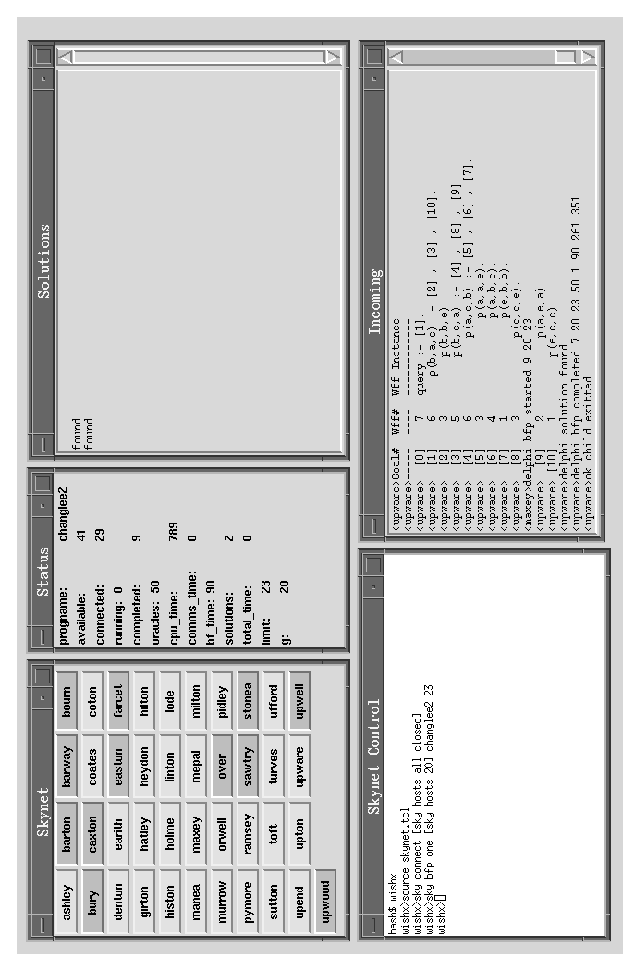
\psfig{file={system/ps/skynet_half_grey.ps}} \hfill}
\caption{Skynet control processor user interface.}
\vspace{5mm}
\label{skynet_half_grey}
\end{figure}

The window labelled ``Skynet Control'' is the command-line interface to skynet,
providing commands such as \texttt{sky\_{}connect} to establish connection with a
\texttt{ppc} daemon, and \texttt{sky\_{}bfp} to initiate the breadth-first
partitioning strategy on all the selected path processors.

The window labelled ``Status'' accumulates runtime information as the
distributed execution of the user program progresses.  In particular, the
\texttt{running} field indicates the number of path processors currently 
executing the user program, and \texttt{completed} shows the number of
path processors which have completed their search and become idle.

The ``Solutions'' window simply displays solutions as they are returned from the
path processors.  The ``Incoming'' window displays the complete log of all communications
from all the path processors.  In the example shown, the solution returned by the
user program is the atom \texttt{found}, to reduce the volume of information
accumulated in the ``Solutions'' window.  The voluminous solution is recorded in
the ``Incoming'' log.

The ``Skynet'' window is a graphical display of the status of each of the
available path processors.  Each button is displayed in one of four colours:
\begin{description}
\item[Grey: ]{Path processor not yet contacted.  A user click on the button will
    cause \texttt{skynet} to connect to the path processor \texttt{ppc} and change
    the button to yellow, or red if the connection fails.}
\item[Yellow: ]{\texttt{skynet} connected to \texttt{ppc}.  A user click will
    disconnect \texttt{skynet} from the path processor \texttt{ppc} and change the
    button back to grey.}
\item[Green: ]{Path processor is currently busy with user process.  A user click
    will send a command to the path processor \texttt{ppc} to
    \textit{kill} the user process.  The button will change back to yellow when
    confirmation of the child exit is received.}
\item[Red: ]{Path processor unavailable.}
\end{description}
When the user issues the \texttt{sky\_{}bfp} command or the \texttt{sky\_{}bfp\_{}one}
command in the ``Skynet Control'' window, the buttons of the selected path
processors will change from yellow to green and the user processes start
execution.  The buttons return to yellow as the path processors complete their
assigned work.

The process \texttt{skyhub} provides a transparent multiplexing function between
\texttt{skynet} and the many \texttt{ppc} daemons.  The primary requirement for
the \texttt{skyhub} process was to overcome the 64 socket-connection limit of
the DECstation 3100's used for the research, although in fact never more than
42 were available.  The \texttt{skyhub} process has facilities for the local
storage and manipulation of variables by the controlling \texttt{skynet}, for
a possible future hierarchical implementation of a partitioning strategy.

